%
% This is the LaTeX template file for lecture notes for EE 382C/EE 361C.
%
% To familiarize yourself with this template, the body contains
% some examples of its use.  Look them over.  Then you can
% run LaTeX on this file.  After you have LaTeXed this file then
% you can look over the result either by printing it out with
% dvips or using xdvi.
%
% This template is based on the template for Prof. Sinclair's CS 270.

\documentclass[twoside]{article}
\usepackage{graphics}
\setlength{\oddsidemargin}{0.25 in}
\setlength{\evensidemargin}{-0.25 in}
\setlength{\topmargin}{-0.6 in}
\setlength{\textwidth}{6.5 in}
\setlength{\textheight}{8.5 in}
\setlength{\headsep}{0.75 in}
\setlength{\parindent}{0 in}
\setlength{\parskip}{0.1 in}

%
% The following commands set up the lecnum (lecture number)
% counter and make various numbering schemes work relative
% to the lecture number.
%
\newcounter{lecnum}
\renewcommand{\thepage}{\thelecnum-\arabic{page}}
\renewcommand{\thesection}{\thelecnum.\arabic{section}}
\renewcommand{\theequation}{\thelecnum.\arabic{equation}}
\renewcommand{\thefigure}{\thelecnum.\arabic{figure}}
\renewcommand{\thetable}{\thelecnum.\arabic{table}}

%
% The following macro is used to generate the header.
%
\newcommand{\lecture}[4]{
   \pagestyle{myheadings}
   \thispagestyle{plain}
   \newpage
   \setcounter{lecnum}{#1}
   \setcounter{page}{1}
   \noindent
   \begin{center}
   \framebox{
      \vbox{\vspace{2mm}
    \hbox to 6.28in { {\bf EE 382C/361C: Multicore Computing
                        \hfill Fall 2016} }
       \vspace{4mm}
       \hbox to 6.28in { {\Large \hfill Lecture #1: #2  \hfill} }
       \vspace{2mm}
       \hbox to 6.28in { {\it Lecturer: #3 \hfill Scribe: #4} }
      \vspace{2mm}}
   }
   \end{center}
   \markboth{Lecture #1: #2}{Lecture #1: #2}
   %{\bf Disclaimer}: {\it These notes have not been subjected to the
   %usual scrutiny reserved for formal publications.  They may be distributed
   %outside this class only with the permission of the Instructor.}
   \vspace*{4mm}
}

%
% Convention for citations is authors' initials followed by the year.
% For example, to cite a paper by Leighton and Maggs you would type
% \cite{LM89}, and to cite a paper by Strassen you would type \cite{S69}.
% (To avoid bibliography problems, for now we redefine the \cite command.)
% Also commands that create a suitable format for the reference list.
\renewcommand{\cite}[1]{[#1]}
\def\beginrefs{\begin{list}%
        {[\arabic{equation}]}{\usecounter{equation}
         \setlength{\leftmargin}{2.0truecm}\setlength{\labelsep}{0.4truecm}%
         \setlength{\labelwidth}{1.6truecm}}}
\def\endrefs{\end{list}}
\def\bibentry#1{\item[\hbox{[#1]}]}

%Use this command for a figure; it puts a figure in wherever you want it.
%usage: \fig{NUMBER}{SPACE-IN-INCHES}{CAPTION}
\newcommand{\fig}[3]{
			\vspace{#2}
			\begin{center}
			Figure \thelecnum.#1:~#3
			\end{center}
	}
% Use these for theorems, lemmas, proofs, etc.
\newtheorem{theorem}{Theorem}[lecnum]
\newtheorem{lemma}[theorem]{Lemma}
\newtheorem{proposition}[theorem]{Proposition}
\newtheorem{claim}[theorem]{Claim}
\newtheorem{corollary}[theorem]{Corollary}
\newtheorem{definition}[theorem]{Definition}
\newenvironment{proof}{{\bf Proof:}}{\hfill\rule{2mm}{2mm}}

% **** IF YOU WANT TO DEFINE ADDITIONAL MACROS FOR YOURSELF, PUT THEM HERE:
\usepackage{listings}
\usepackage{graphicx}

\begin{document}
%FILL IN THE RIGHT INFO.
%\lecture{**LECTURE-NUMBER**}{**DATE**}{**LECTURER**}{**SCRIBE**}
\lecture{19}{November 1}{Vijay Garg}{Zijiang Yang}
%\footnotetext{These notes are partially based on those of Nigel Mansell.}

% **** YOUR NOTES GO HERE:

% Some general latex examples and examples making use of the
% macros follow.  
%**** IN GENERAL, BE BRIEF. LONG SCRIBE NOTES, NO MATTER HOW WELL WRITTEN,
%**** ARE NEVER READ BY ANYBODY.
\section{Wait Free Consensus Hierarchy}
Consensus number of a shared object is the maximum number of processes that can use that object to solve consensus problem. Different objects have different consensus numbers, as shown in the following table.

\begin{center}
    \begin{tabular}{| c | c |}
    \hline
    \textbf{Object Type} & \textbf{Consensus Number} \\ \hline
    Read\&Write & 1 \\ \hline
    Queue(Stack), Test\&Set, Swap, Get\&Increment, (2,1)Objects & 2  \\ \hline
    ... & ... \\ \hline
    Check\&Set & Infinity  \\
    \hline
    \end{tabular}
\end{center}

Based on the hierarchy of consensus objects, we can always use objects with higher consensus number to build objects with lower consensus numbers.

\subsection{Read-Modify-Write Objects}

A Read-Modify-Write object is the abstraction of an general object that has the following structures:

\begin{center}
    \begin{lstlisting}[language=Java]
        private int value; 
        public int synchronized getAndModify(int x) {
            int prev = value;
            value = f(value, x);
            return prev;
        }
    \end{lstlisting}
\end{center}

Each Read-Modify-Write object has an associated value and an atomic operation. The operation will set a new value based on function f and return the old value. 

There are a lot of consensus objects which can be viewed as Read-Modify-Write object. Each has its own f function definition:
\begin{itemize}
  \item Test\&Set: f(v, x) = 1
  \item Swap: f(v, x) = x
  \item Get\&Increment: f(v, x) = v + 1
\end{itemize}

Read-Modify-Write objects can be characterized by the property of funtion f:
\begin{itemize}
  \item A Read-Modify-Write object is commute if \\ \textit{fi fj = fj fi} \\ where \textit{fi} is the funtion applied by process i
  \item A Read-Modify-Write object is overwrite if \\ \textit{fi(fj(x)) = fi(x)   for any i, j} \\ where \textit{fi} is the funtion applied by process i
\end{itemize}

\subsection{Consensus Number of Read-Modify-Write Object}

A \textbf{trivial} Read-Modify-Write object is an Read-Modify-Write object whose f(v, x) = v. It can be viewed as a simple read operation. 

\textbf{Theorem:} Any non-trivial Read-Modify-Write object with either commuting or overwriting property has consensus number equal to two. 

\textbf{Proof:}
\begin{enumerate}
  \item Firstly we need to prove that consensus number for RMW object is at least 2. 
  
           It is easy to come up with an algorithm to solve consensus problem on 2 processes using the non-triviality property: \\
           \begin{center}
               \begin{lstlisting}
                   int[2] A, RMW r (init null)
                   Pi: write proposol on A[i]
                        value = r.getAndModify(i)
                        if(value == null) {
                            I win
                        } else {
                            other process win
                        }
               \end{lstlisting}
           \end{center}
           This algorithm works because the RMW object is non-trivial. Thus there exist v such that f(v, x) != v.
    \item Then we need to prove that the consensus number of RMW object is at most 2.  
    
             We can show that there is not a protocol that solves consensus for 3 processes using RMW objects. \\
             \begin{center}
                 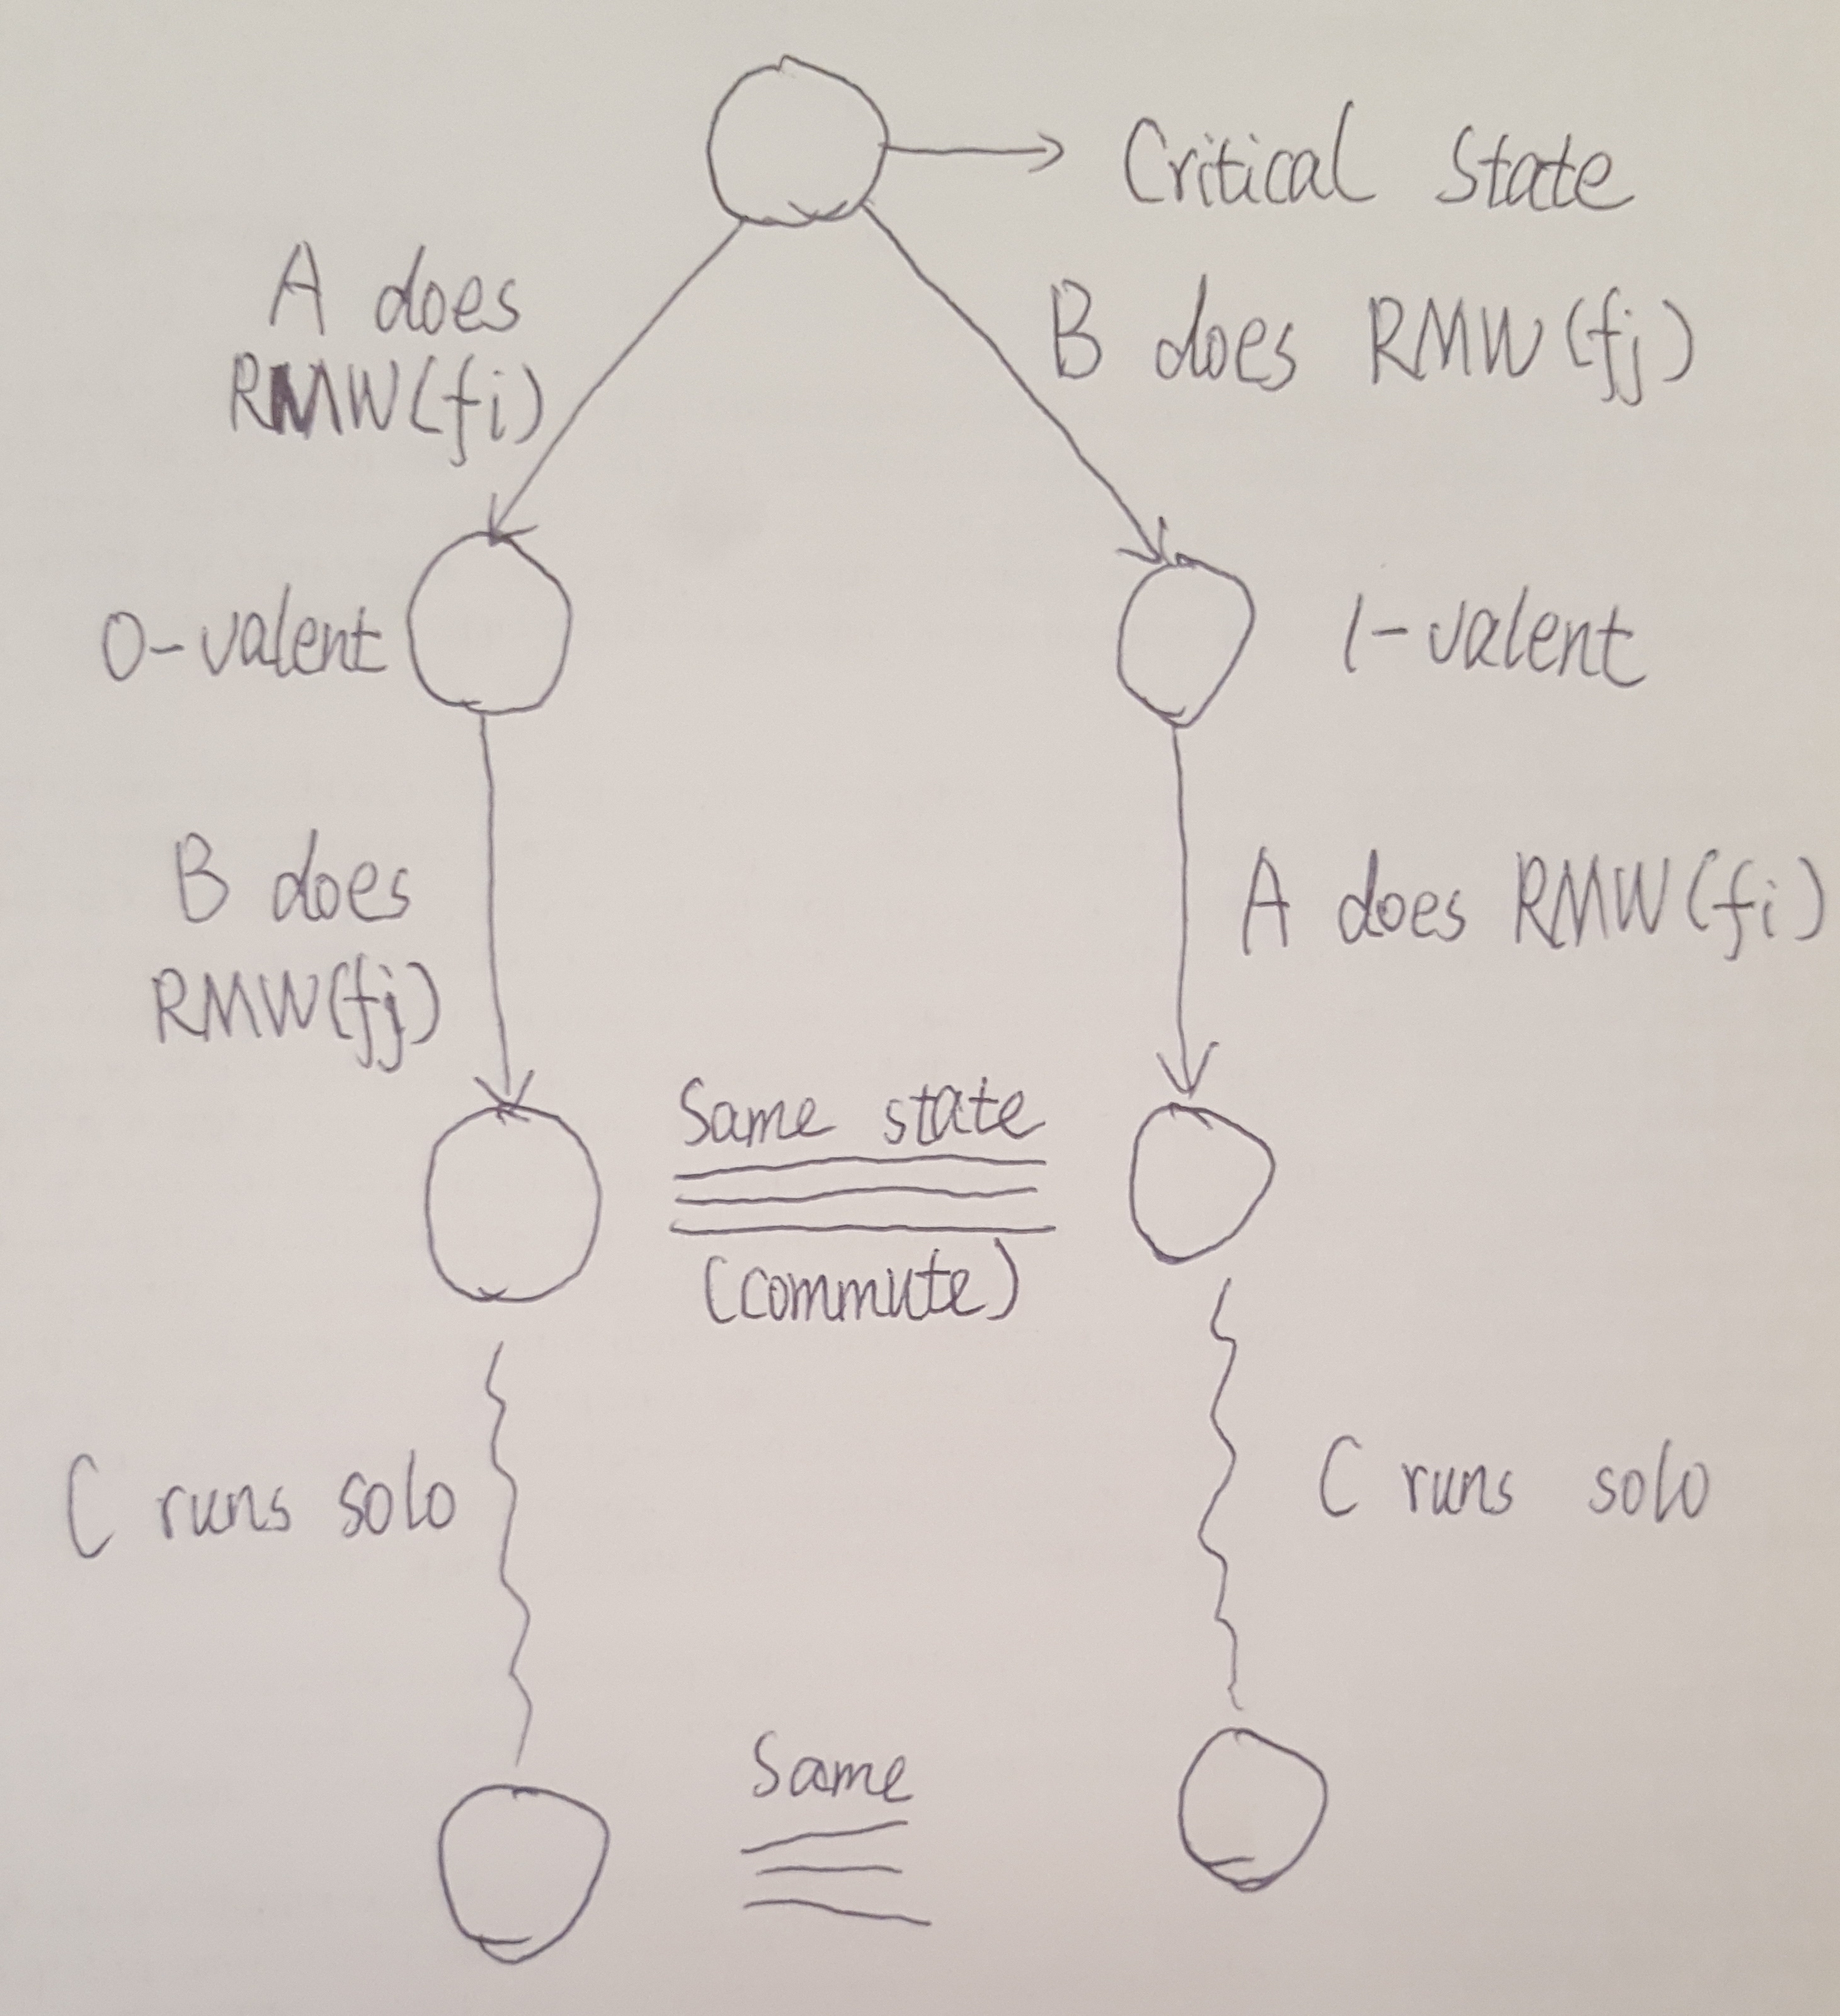
\includegraphics[scale=0.1]{figure1}
             \end{center} 
             In order to reach consensus, a protocol has to reach critical state. Suppose at critical sate A does RMW(fi) and reach to 0-valent state; B does RMW(fj) and reach to 1-valent state. Then at the 0-valent state B does RMW(fj); at the 1-valent state A does RMW(fi). After that, both path reaches the same state. Then C runs solo and will decide the same value from both state. But it contradicts the assumption that one state is 0-valent state and the other state is 1-valent state. Thus it is impossible to reach a critical state for RMW object on 3 processes. 
\end{enumerate}

Thus in conclusion, non-trivial Read-Modify-Write object with either commuting or overwriting property has consensus number equal to two.

\subsection{2-Writes-1-Read Object}

We already know that we cannot use atomic read-write register to solve consensus problem. However we can solve this problem if we are allowed to write 2 locations atomically. A 2-Writes-1-Read object (\textit{(2, 1) object}) is an object which can write 2 locations and read 1 location atomically. 

Following is a protocol that can solve 2 process consensus problem using (2, 1) object.

\begin{center}
    \begin{lstlisting}
        int[3] A, init null
        P0: A[0] = a, A[1] = a (atomically)
        P1: A[1] = b, A[2] = b (atomically)
        whichever writes first wins
    \end{lstlisting}
\end{center}

There are 4 possible configurations:

\begin{itemize}
    \item {[a, a, null]} =\textgreater p0 wins
    \item {[a, b, b]} =\textgreater p0 wins
    \item {[null, b, b]} =\textgreater p1 wins
    \item {[a, a, b]} =\textgreater p1 wins
\end{itemize}

In this way we can solve consensus on 2 processes.

\section{Universal Constructions}

\textbf{Deterministic Object:} given a state and an operation, the resulting state is deterministic.

What we want to do is given some objects of consensus number m, construct a deterministic object with consensus number m' \textless= m.

An easy way would be to use a consensus object to decide who wins. However, in general consensus objects are not reusable.

The correct way would be use a linked list to record the invocation histories, and maintain a consensus object inside each node. When multiple processes wants to invoke methods, use consensus object of the head node to decide which thread wins.

The linked list is organized as follows:

\begin{center}
    \begin{lstlisting}
    Initial state -> apply method1 -> apply method2 -> apply method3
    \end{lstlisting}
\end{center}

The invocation log is equivalent to the current state of the object.

Sudo code can be found in https://github.com/vijaygarg1/UT-Garg-EE382C-EE361C-Multicore/tree/master/chapter7-consensus

\section{Hashing}

Hashing is a technology to map an object into an index. A HashTable uses hashing to decide where to store an item. The time complexity of HashTable is as follows:

\begin{center}
    \begin{tabular}{| c | c |}
    \hline
    \textbf{Operation} & \textbf{Time Complexity} \\ \hline
    Insert & Average O(1) \\ \hline
    Search & Average O(1)  \\ \hline
    Remove & Average O(1)  \\
    \hline
    \end{tabular}
\end{center}

However, generally HashTable may has collisions which may damage the performance. We want to make collisions as infrequent as possible. There are different strategies in case of collision:

\begin{itemize}
    \item \textbf{Chaining:} Store a linked list in each bucket. Add items into the linked list.
    \item \textbf{Open Addressing:}
        \begin{itemize}
            \item Linear Probing: if the bucket h(i) is occupied, insert item into the next available bucket. This approach may cause clustering effect.
            \item Quadratic Probing: if the bucket h(i) is occupied, then try \begin{math}h(i) + 1\end{math}. If still occupied, try \begin{math}h(i) + 2^2\end{math}, then \begin{math}h(i) + 3^2\end{math}, then \begin{math}h(i) + 4^2\end{math} \ldots
        \end{itemize}
\end{itemize}

We want to parallelize the chaining HashTable using lock. A naive solution is to hold a lock for all buckets and acquire the lock for all the operations. A better solution is to hold a lock for every bucket, thus we can parallelize the operations on different buckets. However this approach will waste a lot of spaces. An improvement would be hold a lock for every k buckets. Thus we can save a lot of space while maintain the parallel ability.






\end{document}





